To numerically solve a set of PDEs, iterative methods (finite difference, finite volume or finite element methods) are frequently used to approximate the solution through a discretized (step by step) phenomena. Thus, the continuous time and space domains are discretized so that a set of numerical computations are iteratively (time discretization) applied onto a mesh (space discretization). In other words, the PDEs are transformed to a set of numerical computations applied at each time step on elements of the discretized space domain. Among those numerical computations are found a set of numerical schemes, also called \textit{stencil computations}, a set of auxiliary computations also called \emph{local computations}, and finally a set of \emph{reductions} to reduce a bunch of values to a single scalar value. In the rest of this paper, we denote a \emph{stencil kernel} as a discretized explicit numerical schemes which involve neighborhood computations, whatever the type of space discretization is (mesh).

This section gives a complete formal description of what we call a \textit{stencil program} and its computations. In this paper, the proposed language MSL (Multi-Stencil Language) does not depend on the type of space discretization used. Thus, some details given in the following sections, are usefull to understand the domain but do not have to be kept in mind to understand the Multi-Stencil Language. As a result, at the end of each subsection a summary of what is usefull to understand the language is given.

%-------------------------------------
\subsection{Time, mesh and data}

$\Omega=\mathbb{R}^n$ is the continuous space domain of a numerical simulation. %For example, if $n=3$, any geographic point on earth could be represented in this space in a given geographic coordinate system.
A mesh $\mathcal{M}$ defines the discretization of the continuous space domain $\Omega$ of a set of PDEs and is defined as follows.

\begin{mydef}
A mesh is a connected undirected graph $\mathcal{M}=(V,E)$, where $V\subset \Omega$ is the set of vertices and $E\subseteq V^2$ the set of edges. The set of edges $E$ of a mesh $\mathcal{M}=(V,E)$ does not contain bridges. It is said that the mesh is applied onto $\Omega$.
\end{mydef}
\begin{figure}[!h]\begin{center}
  \resizebox{8cm}{!}{\includegraphics{./images/maillages.pdf}}
  \caption{From left to right, Cartesian, curvilinear and unstructured meshes.}
  \label{fig:mesh1}
\end{center}\end{figure}
\begin{mydef}
The dimension of a mesh $\mathcal{M}=(V,E)$ applied onto $\Omega=\mathbb{R}^n$ is denoted $dim(\mathcal{M})=n$.
\end{mydef}
A mesh can be structured (as Cartesian or curvilinear meshes), unstructured, regular or irregular (without the same topology for each element) as illustrated in Figure~\ref{fig:mesh1}. One can notice that more than one type of mesh is also possible inside a single simulation. For example, an hybrid mesh can be defined as an unstructured mesh composed itself of a Cartesian mesh inside each of its vertices. Multi-grid numerical methods is another example. However, in this paper a single mesh simulation is addressed.

\medskip
\noindent \textbf{Definitions (mesh)}
%\begin{mydef}
\begin{itemize}
\item An entity $\phi$ of a mesh $\mathcal{M}=(V,E)$ is defined as a subset of its vertices and edges, $\phi\subset V\cup E$.
\item A group of mesh entities, denoted $\mathcal{G}$, is a set of mesh entities which are composed of the same topology and types of elements in $V\cup E$.
\item The set of mesh entities groups of a simulation is denoted $\Phi$.
\item Finally, the mesh on which is applied a group of mesh entities $\mathcal{G}$ is denoted $mesh(\mathcal{G})$
\end{itemize}
%\end{mydef}

For example, in a 2D Cartesian mesh an entity could be a cell, made of four vertices and four edges, or simply a vertex. As a result, a group of cells and a group of vertices could be defined in $\Phi$. %This type can be defined as the sets containing exactly four vertices and four edges connected as a cycle. Another type of entities simply are the vertices ($V$) and can be defined as all singletons formed of a single vertex of $V$.

\medskip
This covers the space discretization, however there is also the time dimension which has to be discretized to perform a numerical simulation.

\begin{mydef}
We denote a scalar as a numerical variable. The set of scalars is denoted $\mathcal{S}$.
\end{mydef}

\medskip
\noindent \textbf{Definitions (time)}
%\begin{mydef}
\begin{itemize}
\item $\mathcal{T}=\mathbb{R}$ is the continuous time domain of a numerical simulation.
\item The discretization of the continuous time domain $\mathcal{T}$ is denoted as the pair $T(\Delta t,conv)$.
\begin{itemize}
\item $\Delta t \in \mathcal{S}$ represents the time interval of the numerical simulation, such that for a current time iteration $t_i$, the next time iteration is $t_{i+1} = t_i + \Delta t$.
\item $conv:\mathcal{S}^n \rightarrow bool$ is a function which returns a boolean from a set of scalar variables. This function represents the convergence criteria of the simulation. 
\end{itemize}
\end{itemize}

At a given time step, the convergence criteria is evaluated such that if $conv$ returns $true$ the next time step $t_{i+1} = t_i + \Delta t$ can start. Otherwise the simulation ends. For example, the simplest $conv$ is typically to have two scalars: $t$ the time, and a constant number of iterations denoted $it$. At each time step $\Delta t=1$, and $conv$ returns the boolean expression $t<it$.
%\end{mydef}

In a numerical simulation, a scalar can be associated to each entity of the mesh. In such a case, a single variable is used and is denoted a quantity.
%A quantityas a set of scalars can be applied onto a mesh with a nil dimension, a set of data elements, or quantities, can be applied onto meshes of dimension superior to zero. Those quantities represent, as well as scalars, the set of values to compute, or to use, for computations.

\medskip
\noindent \textbf{Definitions (quantity)}
%\begin{mydef}
\begin{itemize}
\item A quantity represents a variable applied onto a group of mesh entities $\mathcal{G}$.
\item The set of quantities applied onto the mesh is denoted $\Delta$.
\item In the rest of this paper, the group of mesh entities on which a quantity $\delta$ is mapped is denoted $entity(\delta)=\mathcal{G}_{\delta}$.
\end{itemize}
%\end{mydef}

Another option, closer to the applied mathematics domain, would have been to apply a quantity to each entity of a group $\mathcal{G}$, but also to each time iteration. In this case a single quantity would represents all its occurences over time steps. This solution could be investigated in future work, however the approach chosen in this work is to let the user be aware of the number of data he is using and what exactly for.

\paragraph{\textbf{Summary}} In this subsection have been presented the general formalism of what is a mesh, its entities and groups of entities, of how the time is discretized, and finally of what is a scalar and a quantity. The language presented in this paper, the Multi-Stencil Language, offers a simple way to describe a numerical simulation while being able to automatically extract parallelism. Its aim is to be mesh-agnostic, thus to not have details about the topology of the mesh which is an implementation problem. As a result the details about the mesh topology is not needed in the rest of this paper.

%-----------------------
\subsection{Computations}

In this section are considered four different types of kernel computations, stencil kernels, boundary kernels, local kernels, and reduction kernels. 

\medskip
\noindent \textbf{Definitions}
%\begin{mydef}
\begin{itemize}
\item A computation domain $D$ is a subpart of a mesh entities group, $D \subseteq \mathcal{G} \in \Phi$.
\item The set of computation domains of a numerical simulation is denoted $\mathcal{D}$.
\item A neighborhood $n$ is a function which for a given entity $\phi \in \mathcal{G}_i$, returns a set of $m$ entities in $\mathcal{G}_j$, $n : \mathcal{G}_i \rightarrow \mathcal{G}_j^m$. One can notice that $i = j$ is possible. Most of the time, such a neighborhood is called a \emph{stencil shape}.
\item The set of neihborhood functions in a numerical simulation is denoted $\mathcal{N}$.
\end{itemize}

\begin{mydef}
A computation kernel $k$ of a numerical simulation is defined as $k(S,R,(w,D),comp)$, where 
\begin{itemize}
\item $S \in \mathcal{S}$ is the set of scalar to read, 
\item $(w,D) \in \Delta \times \mathcal{D}$ is the single data modified by the computation kernel onto a given computation domain. Thus, $w \in \Delta$ and $D \in \mathcal{D}$ is the computation domain on which $w$ is computed, $D \subseteq \mathcal{G}_w=entity(w)$.
\item $R$ is the set of tuples $(r,n)$, where $r \in \Delta$ and $n \in \mathcal{N}$ is a neighborhood function such that $n : \mathcal{G}_w \rightarrow entity(r)^m$. The neighborhood indicates which entities of $r$ will be read in order to compute a single entity of $w$. 
\item $comp$ is the numerical computation which returns a value from a set of $n$ input values, $comp: V^n \rightarrow V$, where $V$ is typically $\mathbb{N}$, $\mathbb{Z}$, or $\mathbb{R}$. $comp$ represents the actual numerical expression which is computed by a kernel.
\end{itemize}
\end{mydef}

At each time iteration, a set of computations is performed. During a computation kernel, it can be considered that a set of old states ($t-1$) of quantities are read ($R$), and that a new state ($t$) of a single quantity is written ($w$). In this paper only explicit numerical schemes are considered, thus if we denote by $identity$ the identity function, we have $w \not\in R$ except if $w=(r,identity)$.

Such a definition of a computation kernel offers a large panel of different computations. For example, the four usual types of computations (stencil, local, boundary and reduction) performed into a simulation can be defined as follow :
\begin{itemize}
\item A kernel computation $k(S,R,(w,D),comp)$ is a \emph{stencil kernel} if $\exists (r,n) \in R$ such that $n \neq identity$ .
\item A \emph{boundary kernel} is a kernel $k(S,R,(w,D),comp)$ where $D$ is a specific computation domain at the border of entities, and which does not intersect with any other computation domain.
\item A kernel computation $k(S,R,(w,D),comp)$ is a \emph{local kernel} if $\forall (r,n) \in R$, $n = identity$.
\item A kernel computation $k(S,R,(w,D),comp)$ is a \emph{reduction kernel} if $w$ is a scalar.%, $D=\emptyset$, $R=\{(r,n)\}$ with $n=entity(r)$, and $comp$ is a reduction operation (usually $+$, $-$, $*$, $max$, $min$ etc.).
\end{itemize}

%In our formalism, it is forbidden for a stencil kernel to find $(r,n) \in R$ for which $r=w$ and $n \neq identity$. Actually, if such a property was permitted, implicit numerical schemes would be needed into the simulation, which involves linear solvers. Such a scheme is not a stencil and is over the scope of this paper. The problem does not happened for local kernels as $\forall (r,n) \in R$, $n = identity$. Computations for which this property is authorized are boundary kernels only. This type of kernel is a particular case as it commputes boundary conditions, which represents what should happened outside the space domain but still impact stencil kernels at the next time step.

% \noindent \textbf{Property}
% A kernel for which all data read and written are applied onto a mesh of dimension $0$ is a local kernel.

% \noindent \textbf{Property}
% In a reduction kernel $k(S,R,(w,D),comp)$, $D=entity(w)$ as a single entity exists for a scalar.

%\medskip
%A reduction computation is a computation which reads a single data applied onto a mesh and returns from all its entities a single scalar (mesh with a dimension reduced to zero). 

A reduction is typically used to compute the convergence criteria of the time loop of the simulation. Occasionally reductions can also be used during a time iteration.

% \medskip
% \noindent \textbf{Property}
% Considering a reduction kernel $k(S,R,(w,D),comp)$, $comp$ must be a binary and associative operation on the type $V$, $comp: V \times V \rightarrow V$.

\begin{mydef}
The set of $n$ ordered computation kernels of a numerical simulation is denoted $\Gamma = [k_i]_{0 \leq i \leq n-1}$, such that $\forall k_i,k_j \in \Gamma$, if $i < j$, then $k_i$ is computed before $k_j$.
\end{mydef}

\begin{mydef}
A \textit{multi-stencil program} is defined by the octuplet 
\begin{equation*}
\mathcal{MSP}(\mathcal{M},\Phi,\mathcal{D},\mathcal{N},\Delta, \mathcal{S},T,\Gamma)
\end{equation*}
\end{mydef}

\paragraph{\textbf{Summary}} In this subsection have been presented the general formalism of what is a computation kernel and a multi-stencil program. The language presented in this paper, the Multi-Stencil Language, offers a simple way to describe a numerical simulation while being able to automatically extract parallelism. Its aim is to be mesh-agnostic, as previously described, but also to make a clear separation of concerns between the simulation description and its implementation. As a result, and as already described, details about the topology of the mesh, which is an implementation problem, is not used into the language. Moreover, in a computation kernel $k(S,R,(w,D),comp)$, $comp$ is not used by the language.

\paragraph{\textbf{Example}}
For example, in Figure~\ref{fig:ex1}, assuming that the computation domain (full lines) is denoted $dc1$ and the stencil shape is $n1$, the stencil kernel can be defined as:
\begin{equation*}
R: \{(B,n1)\}, \quad w: A, \quad D: dc1,
\end{equation*}
\begin{equation*}
comp: A(x,y)=B(x+1,y)+B(x-1,y)+B(x,y+1)+B(x,y-1).
\end{equation*}
On the other hand, in the example of Figure~\ref{fig:ex2}, assuming the computation domain is $dc2$ and the stencil shape is $n2$, the stencil kernel is defined as:
\begin{equation*}
R: \{(C,n2),(A,identity)\}, \quad w: A, \quad D: dc2,
\end{equation*}
\begin{equation*}
comp: A(x,y)=A(x,y)+C(x1,y1)+C(x1+1,y1).
\end{equation*}

\begin{figure}
\begin{center}
\subfloat[Mesh and mesh domains.\label{fig:meshbase}]{
\resizebox{8cm}{!}{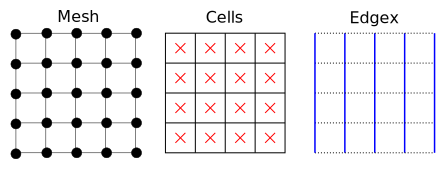
\includegraphics{./images/mesh.pdf}}
}\\
\hspace{10pt}
\subfloat[4-neighborhood stencil.\label{fig:ex1}]{
\resizebox{5cm}{!}{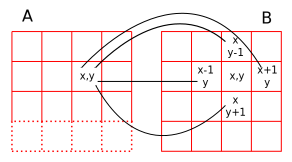
\includegraphics{./images/stencil1.pdf}}
}
\vspace{20pt}
\subfloat[4-neighborhood stencil.\label{fig:ex2}]{
\resizebox{5cm}{!}{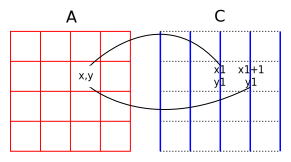
\includegraphics{./images/stencil2.pdf}}
}
\end{center}
\caption{(a) a Cartesian mesh and two kind of mesh entities, (b) an example of stencil kernel on cells, (c) an example of stencil kernel on two different entities of the mesh.}
\label{fig:gspmsp}
\end{figure}

A stencil program has been formally defined in this section. This formalism is used in the next Section to define two parallelization techniques of a multi-stencil program.

One can note that all definitions given in this section are not dependent from the topology of the mesh. This property will be kept in the rest of this paper to propose the mesh-agnostic MSL language.


